\documentclass[t]{beamer}
\usetheme[deutsch]{KIT}
\setbeamercovered{transparent}
\setbeamertemplate{navigation symbols}{}

\KITfoot{Tutoriumsmaterial von Michael Vollmer}
\usepackage[utf8]{inputenc}
\usepackage{amsmath}
\usepackage{ifthen}
\usepackage{amssymb}
\usepackage{tikz}
\usepackage{ngerman}
\usepackage[normalem]{ulem}
\usepackage{stmaryrd}
\usetikzlibrary{automata}
\usenavigationsymbols
\usepackage{mathtools}
\usepackage{array}
\usepackage{colortbl}

\title{Theoretische Grundlagen der Informatik}
\subtitle{Tutorium}
\author{Michael Vollmer}

\institute[IKS]{Institut für Kryptographie und Sicherheit}

\TitleImage[height=\titleimageht]{images/tmaschine.png}

\newcommand{\N}{\ensuremath{\mathbb{N}}}
\newcommand{\M}{\ensuremath{\mathcal{M}}}
\newcommand{\classP}{\ensuremath{\mathcal{P}}}
\newcommand{\classNP}{\ensuremath{\mathcal{NP}}}
\newcommand{\co}{\ensuremath{\mathsf{co\text{-}}}}
\newcommand{\pot}{\ensuremath{\mathcal{P}}}
\newcommand{\abs}[1]{\ensuremath{\left\vert #1 \right\vert}}
\newcommand{\menge}[2]{\ensuremath{\left\lbrace #1 \,\middle\vert\, #2 \right\rbrace}}
\newcommand{\ducttape}[1]{\vspace{#1}}
\newcommand{\neglit}[1]{\overline{#1\vphantom{x^a}}}
\newcommand{\recipe}{\raisebox{-.3cm}{
\includegraphics[scale=.15]{images/chefs-cap.png}}\hspace{0.2cm}}
\newcommand{\opt}[1]{\ensuremath{\text{OPT}(#1)}}
\newcommand{\A}[1]{\ensuremath{\mathcal{A}(#1)}}
\renewcommand{\O}[1]{\ensuremath{\mathcal{O}(#1)}}
\newcommand{\msout}[1]{\text{\sout{\ensuremath{#1}}}}

\newcommand{\invincible}{\setbeamercovered{invisible}} %  "Yesss! I am invincible!!" (Boris Grishenko)
\newcommand{\vincible}{\setbeamercovered{transparent}}
\renewcommand{\solution}[1]{\invincible \pause #1 \vincible}
\newcommand{\micropause}{\\[8pt]}

% \@ifundefined{tikzset}{}{\tikzset{initial text=}} % Text "start" bei Startknoten unterdrücken
\tikzstyle{every node}=[thick]
\tikzstyle{every line}=[thick]

\newcommand{\tutnr}[1]{
  \subtitle{Tutorium #1}
	\begin{frame}
		\maketitle
	\end{frame}
}

\newcommand{\uebnr}[1]{
  \subtitle{Anmerkungen zum #1. Übungsblatt}
	\begin{frame}
		\maketitle
	\end{frame}
}

\begin{document}

\newcommand{\start}[3]
{
  \draw (#1*2,#2*2) node{$#3$};
  \draw (#1*2,#2*2) circle(0.4cm);
  \draw [->] (#1*2-0.9,#2) -- (#1*2-0.4,#2);
}
\newcommand{\final}[3]
{
  \draw (#1*2,#2*2) node{$#3$};
  \draw (#1*2,#2*2) circle(0.4cm);
  \draw (#1*2,#2*2) circle(0.32cm);
}
\newcommand{\startfinal}[3]
{
  \draw (#1*2,#2*2) node{$#3$};
  \draw (#1*2,#2*2) circle(0.4cm);
  \draw (#1*2,#2*2) circle(0.32cm);
  \draw [->] (#1*2-0.9,#2) -- (#1*2-0.4,#2);
}
\newcommand{\state}[3]
{
  \draw (#1*2,#2*2) node{$#3$};
  \draw (#1*2,#2*2) circle(0.4cm);
}
\newcommand{\tol}[4]
{
  \draw (#1+#3,#2*2) node[above]{$#4$};
  \draw [->] (#1*2-0.4,#2*2) -- (#3*2+0.4,#2*2);
}
\newcommand{\tor}[4]
{
  \draw (#1+#3,#2*2) node[above]{$#4$};
  \draw [->] (#1*2+0.4,#2*2) -- (#3*2-0.4,#2*2);
}
\newcommand{\tot}[4]
{
  \draw (#1*2,#2+#3) node[right]{$#4$};
  \draw [->] (#1*2,#2*2+0.4) -- (#1*2,#3*2-0.4);
}
\newcommand{\tob}[4]
{
  \draw (#1*2,#2+#3) node[right]{$#4$};
  \draw [->] (#1*2,#2*2-0.4) -- (#1*2,#3*2+0.4);
}
\newcommand{\totl}[5]
{
  \draw (#1+#3,#2+#4) node[above right]{$#5$};
  \draw [->] (#1*2-0.283,#2*2+0.283) -- (#3*2+0.283,#4*2-0.283);
}
\newcommand{\totr}[5]
{
  \draw (#1+#3,#2+#4) node[above left]{$#5$};
  \draw [->] (#1*2+0.283,#2*2+0.283) -- (#3*2-0.283,#4*2-0.283);
}
\newcommand{\tobl}[5]
{
  \draw (#1+#3,#2+#4) node[below right]{$#5$};
  \draw [->] (#1*2-0.283,#2*2-0.283) -- (#3*2+0.283,#4*2+0.283);
}
\newcommand{\tobr}[5]
{
  \draw (#1+#3,#2+#4) node[below left]{$#5$};
  \draw [->] (#1*2+0.283,#2*2-0.283) -- (#3*2-0.283,#4*2+0.283);
}
\newcommand{\rloopl}[3]
{
  \draw (#1*2-1,#2*2) node[left]{$#3$};
  \draw [->] (#1*2-0.35,#2*2-0.2) arc (-30:-320:0.32cm);
}
\newcommand{\rloopr}[3]
{
  \draw (#1*2+1,#2*2) node[right]{$#3$};
  \draw [->] (#1*2+0.35,#2*2+0.2) arc (150:-140:0.32cm);
}
\newcommand{\rloopt}[3]
{
  \draw (#1*2,#2*2+1) node[above]{$#3$};
  \draw [->] (#1*2-0.2,#2*2+0.35) arc (240:-50:0.32cm);
}
\newcommand{\rloopb}[3]
{
  \draw (#1*2,#2*2-1) node[below]{$#3$};
  \draw [->] (#1*2+0.2,#2*2-0.35) arc (60:-230:0.32cm);
}
\newcommand{\lloopl}[3]
{
  \draw (#1*2-1,#2*2) node[left]{$#3$};
  \draw [->] (#1*2-0.35,#2*2+0.2) arc (30:320:0.32cm);
}
\newcommand{\lloopr}[3]
{
  \draw (#1*2+1,#2*2) node[right]{$#3$};
  \draw [->] (#1*2+0.35,#2*2-0.2) arc (-150:140:0.32cm);
}
\newcommand{\lloopt}[3]
{
  \draw (#1*2,#2*2+1) node[above]{$#3$};
  \draw [->] (#1*2+0.2,#2*2+0.35) arc (-60:230:0.32cm);
}
\newcommand{\lloopb}[3]
{
  \draw (#1*2,#2*2-1) node[below]{$#3$};
  \draw [->] (#1*2-0.2,#2*2-0.35) arc (-240:50:0.32cm);
}
\include{amsmath}

\tutnr{10}

\section{Übungsblatt 4}
\subsection{Übungsblatt 4}

\begin{frame}
\frametitle{Best of Übungsblatt 4}
\begin{itemize}
	\item Abgaben: 13 von 21 (61.9\%)
	\item Mindestens 50\% Punkte: 10 von 13 (76.92\%)
	\item Durchschnittliche erreichte Punktzahl: 8.5
	\begin{itemize}
		\item (nach Aufrunden auf halbe Punkte)
	\end{itemize}
\end{itemize}~\\~\\~\\
Aufgabenverteilung
\begin{enumerate}[{A}ufg{a}be 1:]
	\item Gesamt: 23.75P (durchscnittlich 1.82)
	\item Gesamt: 36.25P (durchschnittlich 2.78)
	\item Gesamt: 14.25P (durchschnittlich 1.1)
	\item Gesamt: 35.25P (durchschnittlich 2.71)
\end{enumerate}
\end{frame}

\section{Reduktion}
\subsection{Reduktion}

\begin{frame}
	\frametitle{NP-Schwere}
	Wie zeige ich, dass $L$ NP-schwer ist?
	\begin{itemize}
		\item Formal: $\forall L' \in NP \colon L' \leq L$
		\begin{itemize}
			\item Das sind ganz schön viele $L'$
		\end{itemize}
		\item Wir nutzen Transitivität der Reduzierbarkeit in polynomieller Zeit
		\begin{itemize}
			\item $\exists L_0 \forall L' \in NP \colon L' \leq L_0 \leq L \Rightarrow L' \leq L$
			\begin{itemize}
				\item $L' \leq L_0$ gilt für alle NP-schweren $L_0$
			\end{itemize}
		\end{itemize}
	\end{itemize}~\\~\\
	Zu zeigen: $\exists L_0 \in NP\text{-schwer} \colon L_0 \leq L \Rightarrow L \in NP\text{-schwer}$
	\begin{itemize}
		\item Erinnerung: $NPC \subset NP\text{-schwer}$
	\end{itemize}
\end{frame}
\begin{frame}
\frametitle{Reduzierung}

\begin{description}
	\item[] $L_0 \leq L$
	\item[$\Leftrightarrow$] Reduziere $L_0$ auf $L$
	\item[$\Leftrightarrow$] $L$ ist mindestens so schwer wie $L_0$
	\item[$\Leftrightarrow$] Ich kann eine Transformation $f \colon L_0 \rightarrow L$ mit folgenden Eigenschaften angeben:
	\begin{itemize}
		\item Die Lösung der erzeugten Instanz induziert eine Lösung der Eingabeinstanz
		\begin{itemize}
			\item Bei Entscheidungsproblem bedeutet dies bspw. dass die erzeugte Instanz genau dann lösbar ist (ein sog. \glqq Ja-Instanz\grqq) wenn die Eingabeinstanz lösbar ist.
		\end{itemize}
		\item Die f ist von geringerer Komplexität als die Probleme
		\begin{itemize}
			\item Bei NP-Problemen darf die Transformation bspw. nur polynomiell Zeit benötigen und muss deterministisch sein.
		\end{itemize}
	\end{itemize}
\end{description}
\end{frame}

\begin{frame}
\frametitle{Bei Entscheidungsproblemen? Gibts noch mehr?}

Die Meisten Entscheidungsprobleme existieren in 3 Formen:
\begin{itemize}
	\item Enscheidungsproblem
	\begin{itemize}
		\item Existiert eine Lösung für das Problem?
		\item \glqq Kann ich diesen Graphen mit 3 Farben färben?\grqq
	\end{itemize}
	\item Suchproblem
	\begin{itemize}
		\item Suche eine Lösung für das Problem
		\item \glqq Wie sieht eine Dreifärbung für diesen Gaphen aus?\grqq
	\end{itemize}
	\item Optimierungsproblem
	\begin{itemize}
		\item Welchen \glqq Grad\grqq\ hat die beste Lösung für dieses Problem?
		\item \glqq Wie viele Farben benötige ich mindestens um den Graphen zu färben?\grqq
	\end{itemize}
\end{itemize}~\\~\\
\begin{itemize}
	\item Umwandlung der Probleme zueinander in der Regel einfach
	\item In dieser Vorlesung hauptsächlich Entscheidungsprobleme
\end{itemize}
\end{frame}

\section{Aufgaben zu P, NP}
\subsection{Aufgabe B10 A2}
\begin{frame}
	\frametitle{Aufgabe B10 A2}
	Finden Sie den Fehler im folgenden ``Beweis'' f"ur \textbf{P} $\not=$ \textbf{NP}!\\
	Betrachten Sie folgenden Algorithmus f"ur SAT:\\[4pt]
	- Durchlaufe f"ur die gegebene Formel $\phi$ alle m"oglichen Belegungen der
	Variablen mit den Wahrheitswerten\\
	- Akzeptiere $\phi$, wenn eine der durchlaufenen Belegungen $\phi$ erf"ullt\\[4pt]
	Dieser Algorithmus hat eine mit der Anzahl der Variablen exponentiell wachsende
	Laufzeit. Daher hat das Problem SAT einen exponentiellen Aufwand und kann nicht in
	\textbf{P} liegen. Weil aber SAT in \textbf{NP} liegt, mu"s also \textbf{P} $\not=$
	\textbf{NP} gelten.
\end{frame}
\subsection{Aufgabe B10 A3}
\begin{frame}
	\frametitle{Aufgabe B10 A3}
	\begin{enumerate}
		\item Zeigen Sie, dass es unter der Voraussetzung \textbf{P} $=$ \textbf{NP} m"oglich
		ist, f"ur eine aussagenlogische Formel $\phi$ in\\
		polynomieller Zeit eine erf"ullende Belegung der Variablen zu finden, falls eine
		solche Belegung existiert!
	\end{enumerate}
\end{frame}

\section{HALF-CLIQUE}
\subsection{HALF-CLIQUE}
\begin{frame}
	\frametitle{HALF-CLIQUE}
	\begin{block}{Wiederholung: CLIQUE}
		Enthält der Graph $G = (V, E)$ einen Teilmenge $V' \subseteq V$ mit $|V'| \geq n$, bei der jeder Knoten eine Kante zu jedem anderen Knoten des Teilgraphs hat?
	\end{block}
	\begin{block}{HALF-CLIQUE}
		Enthält der Graph $G = (V, E)$ eine CLIQUE mit $|V'| \geq |V|/2$?
	\end{block}
\end{frame}
\subsection{Aufgabe B10 A1}
\begin{frame}
	\frametitle{Aufgabe B10 A1}
	Gegeben ist das folgende Problem:
	\begin{tabbing}
	HALF-CLIQUE:\\
	\textit{Gegeben:} \= Ein ungerichteter Graph $G = (V,E)$\\
	\textit{Gesucht:} \> Gibt es eine Teilmenge $V' \subseteq V$\\
	\> mit	$\forall \; v,w \in V', v \not= w: (v,w) \in E$ und $|V'| \geq |V|/2$
	\end{tabbing}
	Beweisen Sie, dass HALF-CLIQUE \textbf{NP}-vollst"andig ist!\\[4pt]
	\underline{Zur Erinnerung:}\\
	Das als \textbf{NP}-vollst"andig bekannte Problem CLIQUE ist definiert durch:
	\begin{tabbing}
	CLIQUE:\\
	\textit{Gegeben:} \= Ein ungerichteter Graph $G = (V,E)$ und $k \in \mathbb{N}$\\
	\textit{Gesucht:} \> Gibt es eine Teilmenge $V' \subseteq V$\\
	\> mit	$\forall \; v,w \in V', v \not= w: (v,w) \in E$ und $|V'| \geq k$
	\end{tabbing}
\end{frame}

\section{Hamiltonkreis und TSP}
\subsection{Hamiltonkreis}
\begin{frame}
	\frametitle{Hamiltonkreis}
	\begin{block}{Kurzdefinition}
	Enthält der gegebene Graph einen Kreis, d.h. gibt es einen Pfad der durch jeden Knoten exakt einmal geht und vom Startknoten wieder zum Startknoten führt (Start- und Endknoten wird nur einmal gezählt).
	\end{block}
	\begin{block}{Formal}
	Gegeben: Ein ungerichteter Graph $G=(V,E)$.\\
	Gesucht: Besitzt $G$ einen Hamiltonkreis? (Dies ist eine Permutation $\pi$ der Knotenindizes ($v_{\pi(1)}$, $v_{\pi(2)}$,...,$v_{\pi(n)}$), sodass für $i=1,...,n-1$ gilt: $\{v_{\pi(i)},v_{\pi(i+1)}\}\in E$) und 
außerdem $\{v_{\pi(n)},v_{\pi(1)}\} \in E)$.
	\end{block}
\end{frame}
\begin{frame}
	\frametitle{Beispiel}
	Gibt es in diesem Graphen einen Hamiltonkreis?
	\begin{center}
		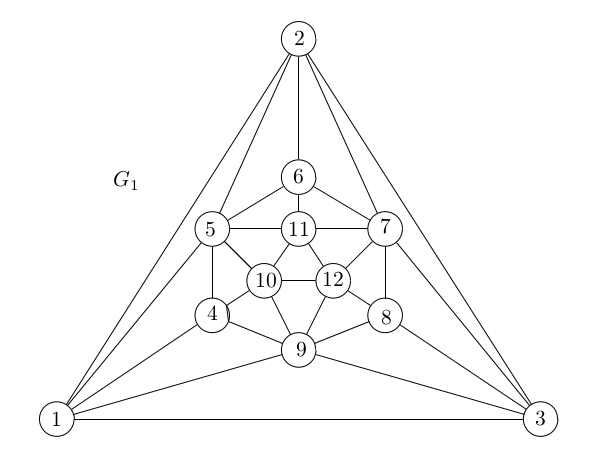
\includegraphics[scale=0.4]{images/4_Faerben}
	\end{center}
\end{frame}
\subsection{Travelling Salesman}
\begin{frame}
	\frametitle{Travelling Salesman}
	\begin{block}{Kurzdefinition}
	Geben sie einen Kreis des gegeben vollständig verbundenen Graphen mit Kantenlängen an, sodass dessen Gesamtkantenlänge minimal ist.
	\end{block}
	\begin{block}{Formal}
	Gegeben: Ein Graph $G=(V,V \times V)$, eine Gewichtungsfunktion $d: V \times V \rightarrow \mathbb{N}$ und ein Parameter $k$\\
	Gesucht: Besitzt $G$ einen einfacher Kreis $C=(v_1,v_2,...,v_n,v_1)$, sodass $n=|V|$ und $\sum_{(u,v)\in C} d(u,v) \leq k$.\\
	\end{block}
\end{frame}
\begin{frame}
	\frametitle{Beispiel}
	Wie lang ist die kürzeste Route und durch welche Kanten geht sie?
	\begin{center}		
		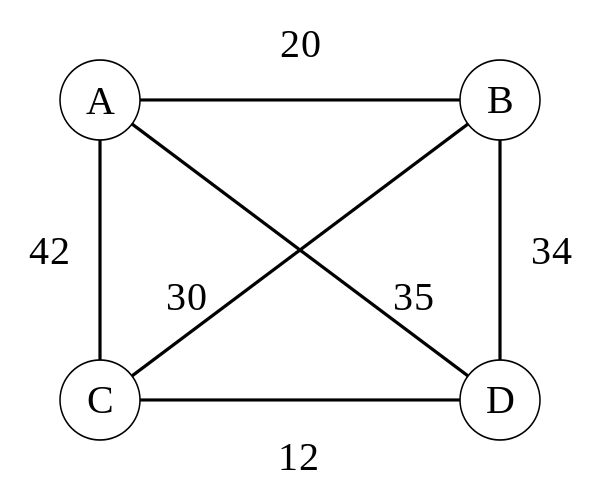
\includegraphics[scale=0.5]{images/Weighted_K4}
	\end{center}
\end{frame}
\subsection{Aufgabe B10 A4}
\begin{frame}
	\frametitle{Aufgabe B10 A4}
 Gegeben sind folgende Probleme: 
	\begin{block}{Hamilton-Kreis}
	Gegeben: Ein ungerichteter Graph $G=(V,E)$.\\
	Gesucht: Besitzt $G$ einen Hamiltonkreis? (Dies ist eine Permutation $\pi$ der Knotenindizes ($v_{\pi(1)}$, $v_{\pi(2)}$,...,$v_{\pi(n)}$), sodass für $i=1,...,n-1$ gilt: $\{v_{\pi(i)},v_{\pi(i+1)}\}\in E$) und 
außerdem $\{v_{\pi(n)},v_{\pi(1)}\} \in E)$.
	\end{block}
\begin{block}{TSP Enscheidungsproblem}
	Gegeben: Ein Graph $G=(V,V \times V)$, eine Gewichtungsfunktion $d: V \times V \rightarrow \mathbb{N}$ und ein Parameter $k$\\
	Gesucht: Besitzt $G$ einen einfacher Kreis $C=(v_1,v_2,...,v_n,v_1)$, sodass $n=|V|$ und $\sum_{(u,v)\in C} d(u,v) \leq k$.\\
	\end{block}
Zeigen Sie, dass TSP NP-Vollständig ist, wobei das Hamiltonkreisproblem auch NP-Vollständig ist. Benutzen Sie für den Beweis die Reduktion Hamiltonkreisproblem$\leq_p$TSP. 
\end{frame}
\begin{frame}
	\frametitle{Aufgabe B10 A4}
Gegeben sei folgender Graph:\newline
\begin{center}
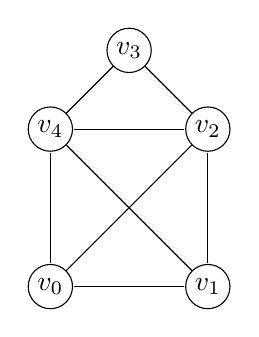
\begin{tikzpicture}
 \draw (0,0) circle (8pt);
 \draw (0,0) node {$v_0$};
 \draw (2,0) circle (8pt);
 \draw (2,0) node {$v_1$};
 \draw (2,2) circle (8pt);
 \draw (2,2) node {$v_2$};
 \draw (1,3) circle (8pt);
 \draw (1,3) node {$v_3$};
 \draw (0,2) circle (8pt);
 \draw (0,2) node {$v_4$};
 \draw (0.2,0.2) -- (1.8,1.8);
 \draw (0.2,1.8) -- (1.8,0.2);
 \draw (0.2,2.2) -- (0.8,2.8);
 \draw (1.2,2.8) -- (1.8,2.2);
 \draw (0.3,0) -- (1.7,0);
 \draw (0.3,2) -- (1.7,2);
 \draw (0,0.3) -- (0,1.7);
 \draw (2,0.3) -- (2,1.7);
\end{tikzpicture}
\end{center}
Gibt es einen Hamiltonkreis? Wandeln Sie hierzu das Problem in ein TSP um und finden Sie eine optimale Rundtour.
\end{frame}
\begin{frame}
	\frametitle{Immer hilfreich: Mehr Probleme}
	\begin{itemize}
		\item NP-Probleme
		\begin{itemize}
			\item Sat
			\item n-Sat ($n \geq 3$)
			\item n-Color ($n \geq 3$)
			\item Partition
			\item Clique
			\item Bin-Packing
			\item Traveling Salesman (TSP)
			\item Knapsack
			\item Vertex Cover
			\item Dominating Set
			\item Independent Set
			\item Hamilton Kreis
			\item Super Mario Bros.
		\end{itemize}
	\end{itemize}
\end{frame}
\section{Schluss}
\subsection{Schluss}
\begin{frame}
\frametitle{Bis zum nächsten Mal!}
\begin{center}
	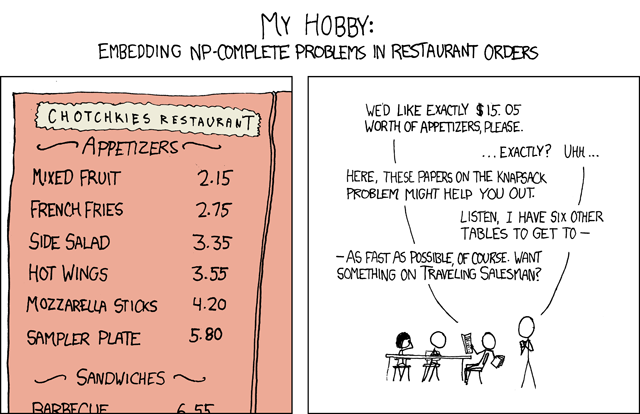
\includegraphics[scale=5.2]{images/287_np_complete.png}
\end{center}
\end{frame}

\frame{
  \frametitle{Lizenzen}
  \center
  
\includegraphics[width=2em]{images/by}
  
\includegraphics[width=2em]{images/cc}
  
\includegraphics[width=2em]{images/sa}
  \\
  {\tiny

Dieses Werk ist unter einem ``Creative Commons Namensnennung-Weitergabe unter gleichen Bedingungen 3.0 Deutschland``-Lizenzvertrag lizenziert. Um eine Kopie der Lizenz zu erhalten, gehen Sie bitte zu \href{http://creativecommons.org/licenses/by-sa/3.0/de/}{http://creativecommons.org/licenses/by-sa/3.0/de/} oder schreiben Sie an Creative Commons, 171 Second Street, Suite 300, San Francisco, California 94105, USA.\\
  \vspace{1cm}
  Davon ausgenommen sind das Titelbild, welches aus der März-April 2002 Ausgabe von American Scientist erschienen ist und ohne Erlaubnis verwendet wird, sowie das KIT Beamer Theme. Hierfür gelten die Bestimmungen der jeweiligen Urheber.
  \vspace{1cm}
  \\ 
  }
  %Habe hier die Reihenfolge etwas umgestellt, weil die Formatierung bei mir komisch aussah. 
  %Wenn es bei dir anders ist, kannst du es auch wieder zurückändern, dann haben wir unterschiedliche Kompilieroptionen
}

\end{document}